\documentclass[border=10pt,crop=true]{standalone}
\usepackage{tikz}
\usetikzlibrary{calc,positioning}

\tikzset{
  opfig/.style={font=\small},
  opfigThin/.style={font=\scriptsize},
  block/.style={
    draw, thick, rounded corners=2pt,
    minimum height=0.9cm, align=center, opfig,
    inner sep=4pt,
  },
  wire/.style={thick},
}

\begin{document}
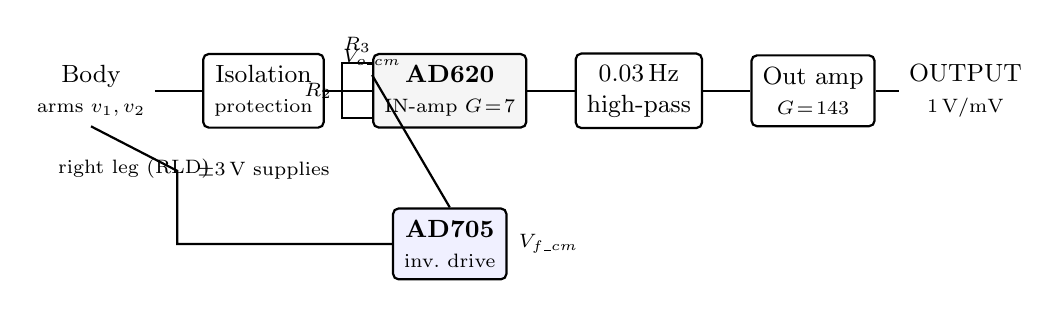
\begin{tikzpicture}[node distance=0.5cm and 0.6cm]

  \node[opfig, align=center] (body) {Body\\{\scriptsize arms $v_1,v_2$}};
  \node[block, right=of body, minimum width=1.5cm] (iso)
    {Isolation\\{\scriptsize protection}};

  \node[block, right=of iso, minimum width=1.35cm, fill=gray!8] (ina)
    {\textbf{AD620}\\{\scriptsize IN-amp $G\!=\!7$}};

  % CM sense R3--R2
  \coordinate (cmMid) at ($(ina.west)+(0,0.2)$);
  \draw[wire] ($(ina.west)+(0,0.35)$) -- ++(-0.38, 0)
    node[midway, above, opfigThin] {$R_3$}
    -- ++(0, -0.7)
    node[midway, left, opfigThin] {$R_2$}
    -- ++(0.38, 0);
  \node[opfigThin, anchor=south] at (cmMid) {$V_{o\_cm}$};

  \node[block, below=1.0cm of ina, minimum width=1.3cm, fill=blue!6] (rld)
    {\textbf{AD705}\\{\scriptsize inv.\ drive}};
  \draw[wire] (cmMid) -- (rld.north);
  \node[opfigThin, right=0.02cm of rld] {$V_{f\_cm}$};

  \node[block, right=of ina, minimum width=1.4cm] (hp)
    {0.03\,Hz\\high-pass};
  \node[block, right=of hp, minimum width=1.2cm] (outa)
    {Out amp\\{\scriptsize $G\!=\!143$}};
  \node[opfig, right=0.3cm of outa, align=center] (out) {OUTPUT\\{\scriptsize 1\,V/mV}};

  \draw[wire] (body) -- (iso) -- (ina) -- (hp) -- (outa) -- (out);

  \coordinate (legJ) at ($(iso.south)!0.5!(body.south)-(0,0.55)$);
  \draw[wire] (rld.west) -| (legJ) -- (body.south)
    node[midway, below, opfigThin] {right leg (RLD)};

  \node[opfigThin, below=0.3cm of iso] {$\pm 3$\,V supplies};

\end{tikzpicture}
\end{document}
